%%%%%%%%%%%%%%%%%%%%%%%%%%%%%%%%%%%%%%%%%
% University Assignment Title Page 
% LaTeX Template
% Version 1.0 (27/12/12)
%
% This template has been downloaded from:
% http://www.LaTeXTemplates.com
%
% Original author:
% WikiBooks (http://en.wikibooks.org/wiki/LaTeX/Title_Creation)
%
% License:
% CC BY-NC-SA 3.0 (http://creativecommons.org/licenses/by-nc-sa/3.0/)
% 
% Instructions for using this template:
% This title page is capable of being compiled as is. This is not useful for 
% including it in another document. To do this, you have two options: 
%
% 1) Copy/paste everything between \begin{document} and \end{document} 
% starting at \begin{titlepage} and paste this into another LaTeX file where you 
% want your title page.
% OR
% 2) Remove everything outside the \begin{titlepage} and \end{titlepage} and 
% move this file to the same directory as the LaTeX file you wish to add it to. 
% Then add \input{./title_page_1.tex} to your LaTeX file where you want your
% title page.
%
%%%%%%%%%%%%%%%%%%%%%%%%%%%%%%%%%%%%%%%%%
%\title{Title page with logo}
%----------------------------------------------------------------------------------------
%   PACKAGES AND OTHER DOCUMENT CONFIGURATIONS
%----------------------------------------------------------------------------------------

\documentclass[12pt]{article}
\usepackage[english]{babel}
\usepackage[utf8x]{inputenc}
\usepackage{amsmath}
\usepackage{commath}
\usepackage{graphicx}
\usepackage[table,xcdraw]{xcolor}
\usepackage[colorinlistoftodos]{todonotes}
\usepackage{placeins}
\usepackage[round]{natbib}
\usepackage{bm}
\usepackage{rotating}
\usepackage{lscape}
\newcommand{\Tfrac}[2]{%
  \ooalign{%
    $\genfrac{}{}{1.2pt}1{#1}{#2}$\cr%
    $\color{white}\genfrac{}{}{.4pt}1{\phantom{#1}}{\phantom{#2}}$}%
}



\begin{document}


\begin{titlepage}

\newcommand{\HRule}{\rule{\linewidth}{0.5mm}} % Defines a new command for the horizontal lines, change thickness here

\center % Center everything on the page

%----------------------------------------------------------------------------------------
%   HEADING SECTIONS
%----------------------------------------------------------------------------------------

%\textsc{\LARGE Aalto University}\\[1.5cm] % Name of your university/college
\textsc{\LARGE T-75.4400 Information retrieval}\\[1.5cm] % Name of your university/college
%\textsc{\Large T-75.4400 Information retrieval}\\[0.5cm] % Major heading such as course name
\textsc{\large Assignment 2}\\[0.5cm] % Minor heading such as course title

%----------------------------------------------------------------------------------------
%   TITLE SECTION
%----------------------------------------------------------------------------------------

\HRule \\[0.4cm]
{ \huge \bfseries On the Efficacy of Alternate Similary Measures, Stemming and Stop Word Removal in 
Text-Based Information Retrieval Systems}\\[0.4cm] % Title of your document
\HRule \\[1.5cm]
 
%----------------------------------------------------------------------------------------
%   AUTHOR SECTION
%----------------------------------------------------------------------------------------

\begin{minipage}{0.45\textwidth}
\begin{center} \large
\textsc{Antti Partanen}\\ % Your name
\texttt{antti.partanen@aalto.fi}\\
295967
\end{center}
\end{minipage}
~
\begin{minipage}{0.45\textwidth}
\begin{center} \large
\textsc{Vikram Kamath}\\ % Supervisor's Name
\texttt{vikram.kamath@aalto.fi}\\
440819
\end{center}
\end{minipage}\\[2cm]


% If you don't want a supervisor, uncomment the two lines below and remove the section above
%\Large \emph{Author:}\\
%John \textsc{Smith}\\[3cm] % Your name



%----------------------------------------------------------------------------------------
%   LOGO SECTION
%----------------------------------------------------------------------------------------


\includegraphics[width=0.2\textwidth]{AaltoSCI_EN_9.pdf}\\[1cm] % Include a department/university logo - this will require the graphicx package
 
%----------------------------------------------------------------------------------------

%----------------------------------------------------------------------------------------
%   DATE SECTION
%----------------------------------------------------------------------------------------

{\large \today}\\[2cm] % Date, change the \today to a set date if you want to be precise
\vfill % Fill the rest of the page with whitespace



\end{titlepage}

%\todo[inline, color=green!40]{Too messy titlepage?}

%\begin{abstract}
%As the amount of data available in electronic form increases continuously, efficient and effective information retrieval techniques are critical. It has been estimated that the amount of data on the Internet doubles every second year. Thus, it is no wonder, that most visible current information retrieval systems are web search engines.

%In this paper, we compare compare two ranking methods: VSM (Vector Space Model) and BM25 for document collection from ACM digital library database. Furthermore, we study the effects of stemmers and stop words. For this study, we use Java with Apache Lucene.  
%\end{abstract}

\section{Introduction}

The task of Information Retrieval (IR) is to obtain information resources, including books, journals and other documents, relevant to the imminent need from a larger collection of information resources. Currently, the most visible information retrieval systems are web search engines. Efficient and effective information retrieval techniques are critical in managing the increasing amount of textual information available in electronic form. Typically, information extraction searches are based on meta-data or full-text indexing.

Automated information retrieval systems are used to reduce the so called \textit{information overload}, i.e. the difficulty of a person to understand an issue due to overwhelming amounts of information. Most of the existing text retrieval techniques rely on indexing key-words, although keywords and index terms alone do not sufficiently capture the documents content. Still, the computational difficulties of more advanced systems keep the keyword indexing as the most viable way by far to process large amount of text. 
The generic textual information retrieval process is show in Figure \ref{fig:IR} and it has the following steps:
\begin{enumerate}
  \item The system builds and index of the documents (\textit{indexing}) 
  \item User describes the \textit{information need} in a form of a query, which is parsed and transformed by the system with the same operations applied to the documents (\textit{query formulation})
  \item The system retrieves, ranks and displays documents that are relevant to the query from the index
  \item User may give relevance feedback to the system
\end{enumerate}
\begin{figure}[ht]
	\centering
	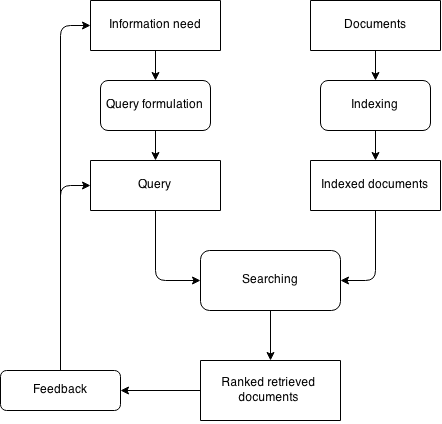
\includegraphics[width=0.8\textwidth]{IR.png}
	\caption{Information retrieval pipeline \citep{hiemstra2009information}}
	\label{fig:IR}
\end{figure}
\FloatBarrier



\subsection{Tools}

We used Java with Apache Lucene, to carry out our experiments. Apache Lucene is a free open source information retrieval software library, developed originally by Doug Cutting in 1999.  Lucene is capable of offering high-performance and includes full-featured text search engine.

\subsection{Content}

In this paper, we compare compare two ranking methods, VSM (Vector Space Model) and BM25 for document collection from ACM digital library database. Furthermore, we analyze what effects does the usage of stemmers (porter stemmer) and stopwords have with the retrieval result. The evaluation of our experiments is visualized with eleven point precision-recall curves. 

\section{Techniques}

Ranking methods are used by search engines to rank matching documents according to their relevance to a given search query. Most common approaches to information retrieval are algebraic (e.g. VSM) and probabilistic (e.g. BM25). The performance of IR methods are usually enhanced by auxiliary methods such as stemming and stopwords.

\subsection{VSM}

VSM (Vector Space Model) is an algebraic representation model for objects as vectors of identifiers. Beyond information retrieval, VSM is also used in information filtering and indexing. The concept of VSM dates back to the early days of information retrieval and it was first utilized in an IR system called SMART \citep{dubin2004most}.

The core idea of VSM is rather simple: represent documents ($D_j$) and queries ($Q$) as vectors of weights \citep{Salton:1975:VSM:361219.361220}.

\begin{equation}
D_j = (w_{1,j}, w_{2,j},...,w_{t,j})
\end{equation}
\begin{equation}
Q = (w_{1,q}, w_{2,q},...,w_{n,q}) 
\end{equation}

There are several different ways of calculating these weights, but \textit{\textbf{tf-idf} (term frequency- inverse document frequency)} is one on the best known. Documents are ranked according to their proximity to the query in this space, where proximity corresponds to the similarity of the vectors. Similarity is not calculated as an euclidean distance, but rather as an cosine between the vectors.

\begin{equation}
cos\theta = \frac{D_j \cdot Q}{\norm{D_j} \norm{Q}}  
\end{equation} 
where
\begin{equation}
\norm{Q} = \sqrt{\sum\limits_{i=1}^n q_i }
\end{equation}
\begin{equation}
\norm{D_j} = \sqrt{\sum\limits_{i=1}^n d_i }
\end{equation}
\begin{equation}
D_j \cdot Q = \sum\limits_{i=1}^n d_i q_i
\end{equation}

\subsection{BM25}

BM25, often referred to as Okapi BM25 (where BM stands for Best Matching), is a probabilistic ranking function. It is based on probabilistic relevance model, devised by \citep{robertson1996okapi}. 

BM25 uses a bag-of-words representation of a document, a representation that ignores the relative ordering of words in the document and the query. It isn't one stand-alone method, but is actually a collection of functions, each of which uses different hyper-parameters, the outputs of which are combined to give the final similarity score between a document and a query. BM25 uses both term frequencies and inverse document frequencies to compute the final similarity score. The BM25 retrieval formula is part of the BM family of retrieval models and according to the Encyclopedia of database systems \citep{amati2009bm25}, it defines the document-query matching function as:

\begin{equation}
 \sum\limits_{t \in q} (k+l)\frac{\bm{tf}}{k+\bm{tf}} \cdot (k_3+ld) \frac{\bm{tf}_q}{k_3 + \bm{tf}_q} \cdot ln\frac{ (r_t +0.5) \cdot (N-R-n_t+r_t+0.5) }{(n_t-r_t+0.5) \cdot (R-r_t+0.5)}
\end{equation}
where
\begin{itemize}
\item $R$ is the number of documents know to be relevant to a specific topic,
\item $r_t$ is the number of relevant documents containing the term,
\item $N$ is the number of documents of the collection, 
\item $n_t$ is the document frequency of the term,
\item $\bm{tf}$ is the frequency of the term in the document,
\item $q$ is the query,
\item $\bm{tf}_q$ is the frequency of the term within the topic from which $q$ was derived
\item $l$ is the document length
\item $k$ is $k_1( ( 1-b ) + b( \Tfrac{l}{1} ) )$
\item $k,1$, $b$ and $k_3$ are parameters which depend on the nature of the queries and possibly the database

\end{itemize}

\subsection{Stemmers}

In most languages and predominantly so in English, words occur in different forms even though they have the same meaning. For example \lq democracy', \lq democratic' , \lq democratize' all have the same derivation and although they're used in different contexts, they have the same \lq semantic' meaning. More often than not, it would be useful to search for using just one of the forms and have documents retrieved that contain all semantically similar forms. Lemmatization is a crude heuristic process that aims to achieve this by removing the ends of the words so that different forms of the same word, after processing, lead to the same, shortened form. So in the example above, all three words would map to ’democraci’ after processing. We used the porter stemmer \citep{porter1980algorithm} for our experiments (although there exist many other different stemming algorithms that aim to achieve a good ’lemmatization’)

\subsection{Stopwords}

Most search engines preprocess both indexed text and search queries so as to remove commonly occurring words that are of little value to the context of the document. Words like \lq A', \lq and',\lq the', \lq of' etc are found abundantly in most English documents but add no overall value to the indexing, ranking or retrieval process. The average size of stopword collections is between 200 - 300 terms \citep{manning2008introduction}. We experimented with using the Lucene in-built stopword list, which although not exhaustive (relative to some of the stop-word corpora available), is sufficiently good. 

\section{Evaluation}

To evaluate the results, we used precision, recall and \textit{11-point precision recall curves}. Precision (a.k.a. positive predictive value) is the fraction of the \textit{retrieved relevant documents to the number of retrieved documents}, whereas recall (a.k.a. sensitivity) is the fraction of the \textit{retrieved relevant documents to all relevant documents} \citep{buckland1994relationship}. If we denote the amount of \textit{relevant documents} with $N_{rel}$ and the amount of \textit{retrieved documents} with $ N_{ret} $, we get the following formulas for precision and recall:

\begin{equation}
precision = \frac{ \abs{ N_{rel} \cap N_{ret} } }{\abs{N_{ret}}}
\end{equation}
\begin{equation}
recall = \frac{ \abs{N_{rel} \cap N_{ret} } }{\abs{N_{rel}}}
\end{equation}

Eleven point precision-recall curve is a graph that plots recall and precision of an information retrieval system at 11 equally spaced recall levels $recall = (0.0, 0.1, 0.2,..., 1.0)$ \citep{zhang2009eleven}. Uninterpolated precision-recall graph typically has a saw-tooth like shape and ideal precision recall curves are flat, so that the curve has the precision value 1 at recall value 1 (the right hand corner). 

We evaluated the systems in the following way. Each query was processed with both methods (VSM and BM25) and the following combination of stopwords and stemmer.

\begin{itemize}
\item No Porter stemmer and no stop words
\item No Porter stemmer and stop words 
\item Porter stemmer and no stop words
\item Porter stemmer with stop words.
\end{itemize}

All in all, each query is processed by a total of 8 different scenarios. The results for each query are plotted in a 11-point precision recall curves shown in the Figures \ref{fig:Query1}, \ref{fig:Query2} and \ref{fig:Query3}. The plots are arranged so, that the VSM plots are on the left-hand side and the BM25 plots are on the right-hand side. On the same row are the VSM and BM25 methods using the same combination of stopwords and stemmer. The rest of the results can be found in Appendix \ref{App:table}. 

%The queries consist of different words. The first query includes words \textit{content}, \textit{based}, \textit{video}, \textit{annotation}. The second query includes  \textit{automatic}, \textit{semiautomatic}, \textit{video}, \textit{tagging} and the third query includes the words \textit{feature}, \textit{based}, \textit{multimedia}, \textit{annotation}. 


\begin{figure}[ht]
  \centering
  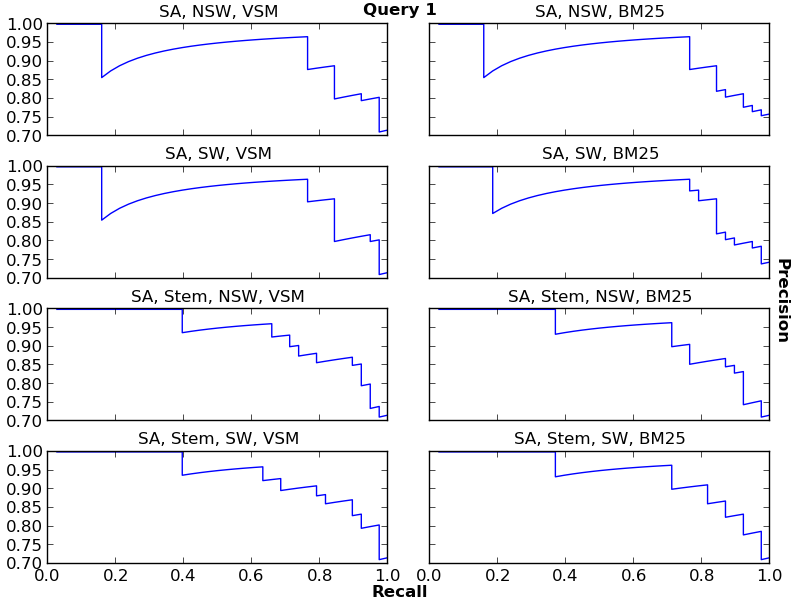
\includegraphics[width=0.8\textwidth]{Query1.png}
  \caption{Query 1 }
  \label{fig:Query1}
\end{figure}
\FloatBarrier

\begin{figure}[ht]
  \centering
  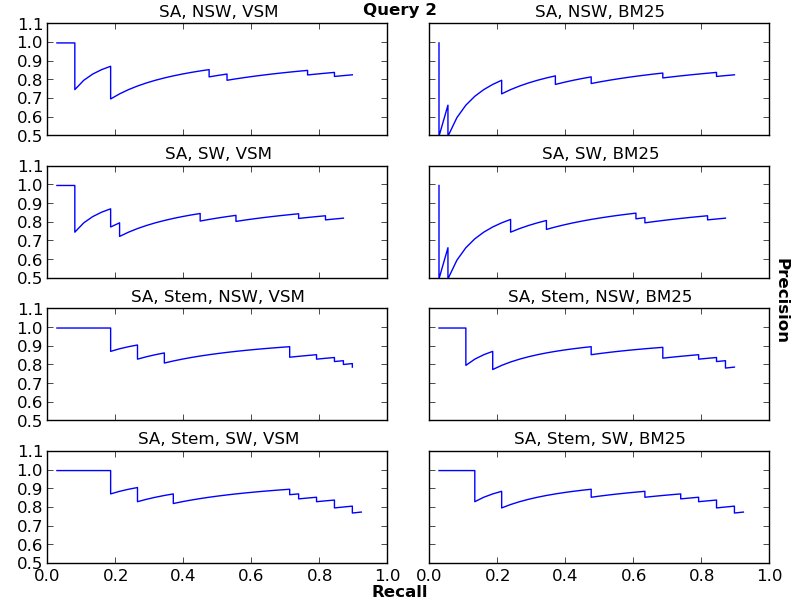
\includegraphics[width=0.8\textwidth]{Query2.png}
  \caption{Query 2 }
  \label{fig:Query2}
\end{figure}
\FloatBarrier

\begin{figure}[ht]
  \centering
  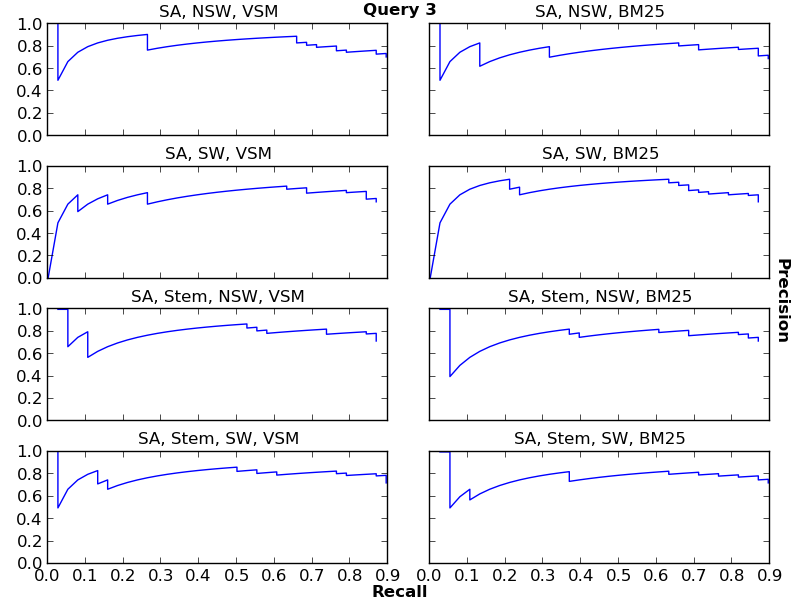
\includegraphics[width=0.8\textwidth]{Query3.png}
  \caption{Query 3 }
  \label{fig:Query3}
\end{figure}
\FloatBarrier


The figures indicate that the usage of porter stemmer increases the precision for the first results. This shows as a step in the precision-recall plots. For example, in the Figure \ref{fig:Query1} the plots with porter stemmer have a precision of 1 for longer than the corresponding plots without the porter stemmer. The same pattern is also noticeable in the Figure \ref{fig:Query2} and in the Figure \ref{fig:Query3}, although it is slightly less visible. These results seem to confirm some earlier observations about the Porter stemmer, i.e. it tends to give consistent (if rather small) performance benefits across a range of collections \citep{croft1994corpus}. 

The usage of stop words seems to have no noticeable effect in any of the queries. There are some differences between the systems using stop words, but these seem to be arbitrary and minuscule. 

Although the ranking order of documents between the two methods were quite different, we were surprised to notice that the different methods have very little difference when plotted against precision-recall plot. Also the F-score values in Table \ref{fig:table} (Appendix \ref{App:table}) are similar for the both methods across the queries and parameters.

We were able to find one anomality in the data, which is in a document titled \lq Enhancing search in a geospatial multimedia annotation system'. It has a relevance of \lq 3', or in other words, it has an undefined relevance value as the relevance should be just a boolean value. We got around it, by marking it as \lq 0'. But, unfortunately, that resulted in noticeable early dips in the query 3 plots (Figure \ref{fig:Query3}) as the methods ranked the document quite high.

\section{Conclusions}

In this paper, we compared two information retrieval methods: VSM and BM25. We also tested what effects does the usage of stemmer and stopwords have on the outcome. We found out that the use of Porter stemmer had the largest influence on the precision-recall curves and, rather surprisingly, the usage of stopwords or the usage of different methods (VSM and BM25) had very little effect on the precision-recall plots of the results. 

One plausible reason for the lack of disparity between the two methods might be in the size of the vocabulary. Since the number of documents relevant to our task (60) doesn't constitute a sizeable vocabulary, the vectors in the vector space model that represent a document are relatively small and dense. If the corpus were larger, say a few hundred or a few thousand documents, the dictionary that represents the number of unique words would be a great deal larger (and considerably sparser), making an inner product in the document space vary much more with the computations that BM25 yields. Despite the relatively small dictionary size, it is expected to see some variability which, albeit minor, is visible in the third query (Appendix \ref{App:table}, Table \ref{fig:table}, rows 17\&18) in the number of documents that were retrieved. 

\section{Contributions}

In the end both of us put equal amounts of effort into the project. We used GitHub for version control and although we did some independent work at the comfort of our own homes, a bulk of the work was done in a series of \lq hackathon' style, caffeine-fueled meetings, where we just sat for 4-6 hours straight at Maari and worked on it. Although this style might be deemed by some as a sloppy, we'd like to think of it as pair programming on speed - in that the fact that we sat together and worked on it enabled almost seamless debugging and ideation.\\

\clearpage

\nocite{*}
\bibliographystyle{myplainnat}
\bibliography{bibliography.bib}


\clearpage
\appendix
\section{Installation instructions} \label{App:instructions}

Here is a brief systems installation and system configuration instructions. 

\begin{enumerate}

\item {\bf Preprocessing} \\
We wrote a small script to parse the XML file and dump \lq items' relevant to our search task
in a document called \lq data.xml'. It is assumed that this file will be used as a command line
argument to the program. To create a fresh dump, run \lq parseXML.py' and ensure that the corpus
file is in the same directory as the script. 
\item {\bf Java Indexing, Search and Ranking Implementation} \\
The whole Java project \lq Assignment2' once loaded into your Eclipse workspace
will make available the file \lq assignment2.java', that contains our implementation. 
Make sure to use all our imports as we use the Java HashMap implementation in our code.
\item {\bf Plotting, Metrics} \\
We dumped the output of \lq assignment2.java' into csv files, one for each query-parameter
combination (24 in total - 8 per query). The csv files, ordered according to query are in
a folder called \lq PrecRec', which further contains 3 folders, one per query containing csv
files relevant to the query. Each of the query folders also contains a python script called \lq calcPrecRecall.py\rq 
that consumes the csv files in the folder and computes the 11-point non-interpolated precision recall curve,
which is then saved into a \lq plot.png' file in the same folder. 
\end{enumerate}


\newpage
\section{Result table} \label{App:table}

\begin{table}[h]
\centering
\resizebox { 1.0\textwidth }{!}{ 
\begin{tabular}{lllllllll}
\rowcolor[HTML]{000000} 
{\color[HTML]{FFFFFF} Query Number} & {\color[HTML]{FFFFFF} Stemmer} & {\color[HTML]{FFFFFF} StopWords} & {\color[HTML]{FFFFFF} VSM/BM25} & {\color[HTML]{FFFFFF} Retrieved} & {\color[HTML]{FFFFFF} Relevant} & {\color[HTML]{FFFFFF} Precision} & {\color[HTML]{FFFFFF} Recall} & {\color[HTML]{FFFFFF} F-Score} \\
\rowcolor[HTML]{EFEFEF} 
1                                   & None                           & No                               & VSM                             & 54                               & 38                              & 0,7037                           & 1                             & 0,826                          \\
\rowcolor[HTML]{EFEFEF} 
1                                   & None                           & No                               & BM25                            & 54                               & 38                              & 0,7037                           & 1                             & 0,826                          \\
\rowcolor[HTML]{EFEFEF} 
1                                   & None                           & Yes                              & VSM                             & 54                               & 38                              & 0,7037                           & 1                             & 0,826                          \\
\rowcolor[HTML]{EFEFEF} 
1                                   & None                           & Yes                              & BM25                            & 54                               & 38                              & 0,7037                           & 1                             & 0,826                          \\
\rowcolor[HTML]{EFEFEF} 
1                                   & Porter                         & No                               & VSM                             & 53                               & 38                              & 0,7169                           & 1                             & 0,8351                         \\
\rowcolor[HTML]{EFEFEF} 
1                                   & Porter                         & No                               & BM25                            & 53                               & 38                              & 0,7169                           & 1                             & 0,8351                         \\
\rowcolor[HTML]{EFEFEF} 
1                                   & Porter                         & Yes                              & VSM                             & 53                               & 38                              & 0,7169                           & 1                             & 0,8351                         \\
\rowcolor[HTML]{EFEFEF} 
1                                   & Porter                         & Yes                              & BM25                            & 53                               & 38                              & 0,7169                           & 1                             & 0,8351                         \\
\rowcolor[HTML]{C0C0C0} 
2                                   & None                           & No                               & VSM                             & 41                               & 34                              & 0,8292                           & 0,8947                        & 0,8607                         \\
\rowcolor[HTML]{C0C0C0} 
2                                   & None                           & No                               & BM25                            & 41                               & 34                              & 0,8292                           & 0,8947                        & 0,8607                         \\
\rowcolor[HTML]{C0C0C0} 
2                                   & None                           & Yes                              & VSM                             & 40                               & 33                              & 0,825                            & 0,8684                        & 0,8461                         \\
\rowcolor[HTML]{C0C0C0} 
2                                   & None                           & Yes                              & BM25                            & 40                               & 33                              & 0,825                            & 0,8684                        & 0,8461                         \\
\rowcolor[HTML]{C0C0C0} 
2                                   & Porter                         & No                               & VSM                             & 43                               & 34                              & 0,7906                           & 0,8947                        & 0,8395                         \\
\rowcolor[HTML]{C0C0C0} 
2                                   & Porter                         & No                               & BM25                            & 43                               & 34                              & 0,7906                           & 0,8947                        & 0,8395                         \\
\rowcolor[HTML]{C0C0C0} 
2                                   & Porter                         & Yes                              & VSM                             & 45                               & 35                              & 0,7777                           & 0,921                         & 0,8433                         \\
\rowcolor[HTML]{C0C0C0} 
2                                   & Porter                         & Yes                              & BM25                            & 45                               & 35                              & 0,7777                           & 0,921                         & 0,8433                         \\
\rowcolor[HTML]{9B9B9B} 
3                                   & None                           & No                               & VSM                             & 48                               & 34                              & 0,7083                           & 0,8947                        & 0,7906                         \\
\rowcolor[HTML]{9B9B9B} 
3                                   & None                           & No                               & BM25                            & 49                               & 34                              & 0,6938                           & 0,8947                        & 0,7816                         \\
\rowcolor[HTML]{9B9B9B} 
3                                   & None                           & Yes                              & VSM                             & 48                               & 33                              & 0,6875                           & 0,8684                        & 0,7674                         \\
\rowcolor[HTML]{9B9B9B} 
3                                   & None                           & Yes                              & BM25                            & 48                               & 33                              & 0,6875                           & 0,8684                        & 0,7674                         \\
\rowcolor[HTML]{9B9B9B} 
3                                   & Porter                         & No                               & VSM                             & 46                               & 33                              & 0,7173                           & 0,8684                        & 0,7857                         \\
\rowcolor[HTML]{9B9B9B} 
3                                   & Porter                         & No                               & BM25                            & 46                               & 33                              & 0,7173                           & 0,8684                        & 0,7857                         \\
\rowcolor[HTML]{9B9B9B} 
3                                   & Porter                         & Yes                              & VSM                             & 47                               & 34                              & 0,7234                           & 0,8947                        & 0,8                            \\
\rowcolor[HTML]{9B9B9B} 
3                                   & Porter                         & Yes                              & BM25                            & 47                               & 34                              & 0,7234                           & 0,8947                        & 0,8                           
\end{tabular}}
\caption{All results}
\label{fig:table}
\end{table}

\FloatBarrier

\end{document}
